\subsection{Imágenes}

Las siguientes implementaciones operan con imágenes del tipo bmp y canales $alfa$, $red$, $green$ y $blue$ ($argb$) de 8 bits cada uno (de ahí la variante bmp 32 bits).\\

En memoria los datos de cada pixel estarán ordenados a la inversa, es decir, $bgra$, por lo cual al trabajarlos en registros de procesador, los mismos serán invertidos debido a que es el formato standard utilizado por la arquitectura intel para almacenar datos en memoria.
El puntero de fuente obtenido en todas las implementaciones representa a la imágen a la cual se le quiere aplicar el filtro. La misma tiene una particularidad para la lectura y es que la primera fila leida es la última de la imágen.\\

Llamaremos $O$ a la imágen de salida generada por cada filtro. Por ejemplo, el filtro identidad
estaría caracterizado por la fórmula\\

\begin{center}
$\forall$ $k$ $\in$ ($r, g, b, a$) $O^{k}_{i,j}$ = $I^{k}_{i,j}$
\end{center}

\subsection{Implementaciones}
Introduciremos cada filtro mencionandolos en el siguiente orden:
 
\begin{enumerate}
\item Cropflip
\item Sepia
\item Low dynamic range 
\end{enumerate}

Para cada uno expondremos su idea principal, es decir, que efecto tiene sobre la imágen a la que se aplica, mostrando un caso de ejemplo. Luego expondremos las implementaciones, focalizando y detallando principalmente la implementación en lenguaje assembler SIMD.

\subsection{Cropflip}
Este filtro es una unión de dos filtros: crop y vertical-flip. Al aplicarlo sobre una imágen, recorta una parte de la misma y la voltea verticalmente. Para ello recibe cuatro argumentos delimitando un rectangulo de la imágen.

\begin{itemize}
\item{$tamx$: Posee la cantidad de columnas, en pixeles, a recortar. Este número es multiplo de 4.}
\item{$tamy$: Contiene la cantidad de filas, en pixeles, a recortar.}
\item{$offseex$: Columna, en pixeles, a partir de la cual se debe comenzar a recortar. Este número también es multiplo de 4.}
\item{$offsety$: Fila, en pixeles, a partir de la cual se debe comenzar a recortar.}
\end{itemize}

El recuadro obtenido se devuelve espejadolo verticalmente. Para ello rearma las filas en orden inverso.\\

\begin{figure}
  \centering
  \subfloat[Original]{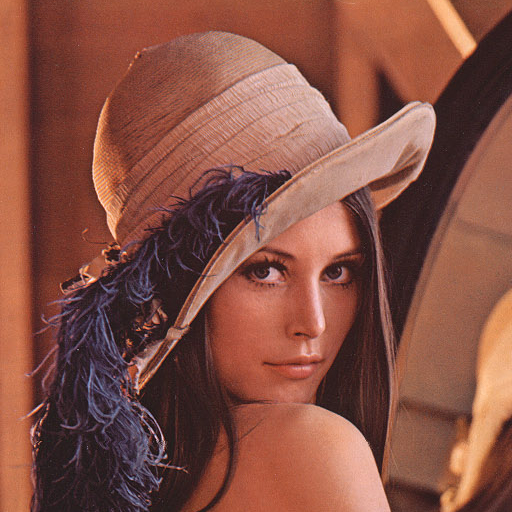
\includegraphics[width=0.4\textwidth]{imagenes/lena32.jpg}\label{fig:f1}}
  \hfill
  \subfloat[Cropflip]{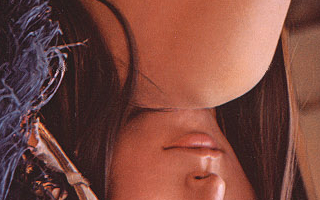
\includegraphics[width=0.4\textwidth]{imagenes/lena32cropflip.jpg}\label{fig:f2}}
  \caption{Corte: 320$x$200 $offset x: 100$ y $offset y: 0$}
\end{figure}

Si bien es el código más sencillo de implementar, incluso de manera eficiente, requiere algún tipo de explicación.

\subsubsection{Assembler SIMD}

En la implementación de SIMD se aprovecha el uso de paralelismo y la capacidad de almacenar hasta cuatro pixeles en un registro $xmm$.\\ 
Tomando entonces de a 4 pixeles, desde el inicio del rectangulo determinado por los parametros, se rearma la imágen, logrando finalmente, al recorrer todas las filas indicadas, el espejado vertical esperado.

\begin{codesnippet}
\begin{verbatim}
.ciclo:
        movdqu xmm1, [rdi]      ; p0|p1|p2|p3
        movdqu [rsi], xmm1
    
        lea rsi, [rsi + 16]
        lea rdi, [rdi + 16]
        loop .ciclo
\end{verbatim}
\end{codesnippet}

Como puede observarse, mediante un ciclo podemos con la ayuda de un registro xmm transportar desde la fuente hasta el destino, 4 pixeles simultaneamente. Esto supondría en principio una ventaja sobre la siguiente implementación.

\subsubsection{C}

Debido a que no disponemos de paralelismo, no nos es posible enviar desde la fuente al destino 4 pixeles simultaneamente. Por lo tanto cada pixel se opera unitariamente. Igualemente se puede llevar a cabo con la ayuda de dos simples ciclos anidados.

\begin{codesnippet}
\begin{verbatim}
	for (int i = 0; i < tamy; i++) 
	{
		for (int j = 0; j < tamx; j++) 
		{

			bgra_t *p_d = (bgra_t*) &dst_matrix[(tamy-1)-i][j*4];
            		bgra_t *p_s = (bgra_t*) &src_matrix[i+offsety][(j+offsetx)*4];

			p_d->b = p_s->b;
			p_d->g = p_s->g;
			p_d->r = p_s->r;
			p_d->a = p_s->a;

		}
	}
\end{verbatim}
\end{codesnippet}

\subsection{Sepia}
Esta operación consiste en cambiar la información de color de cada pixel de la siguiente manera:

\begin{center}
$$O_{i,j}^{R} = 0, 5 . suma_{i,j}$$
$$O_{i,j}^{G} = 0, 3 . suma_{i,j}$$
$$O_{i,j}^{B} = 0, 2 . suma_{i,j}$$
\end{center}

donde 

\begin{center}
$suma_{i,j} = I_{i,j}^{R} + I_{i,j}^{G} + I_{i,j}^{B}$
\end{center}

El efecto logrado es que realza más el canal verde (? soy daltonico y malo pa los colores). 

\begin{figure}
  \centering
  \subfloat[Original]{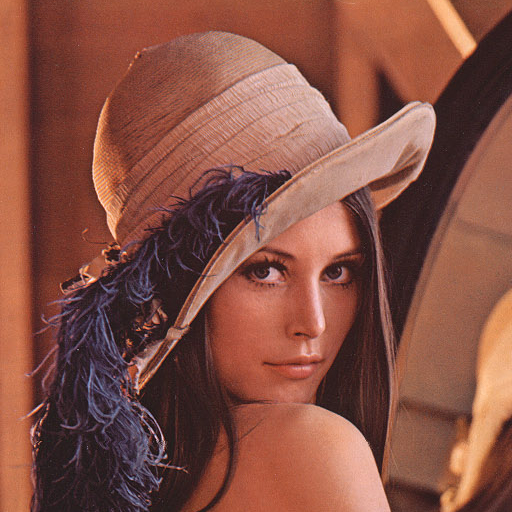
\includegraphics[width=0.4\textwidth]{imagenes/lena32.jpg}\label{fig:f3}}
  \hfill
  \subfloat[Sepia]{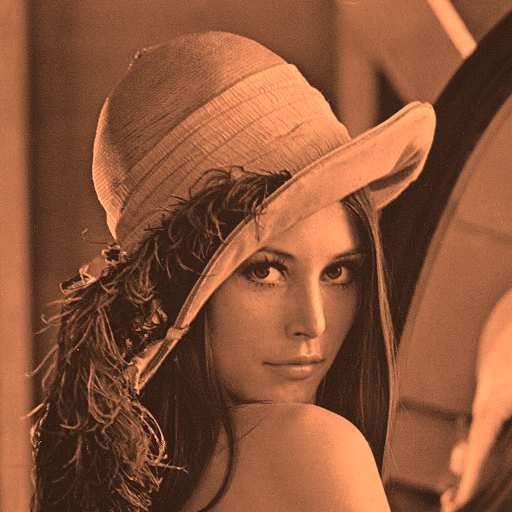
\includegraphics[width=0.4\textwidth]{imagenes/lena32sepia.jpg}\label{fig:f4}}
\end{figure}

Si bien es una operación sencilla, los tiempos de cómputo se ven comprometidos para imágenes muy grandes debido a la cantidad de operaciones en punto flotante: En una imágen de 512$x$512 pixeles tenemos 512$x$512$x$3 = 786432 operaciones de punto flotante. Lo cual puede suponer un desafio si no se dispone de tecnologias como SIMD.

\subsubsection{Assembler SIMD}

Al igual que en el primer filtro, se aprovecha el paralelismo de SIMD y en particular la eficiencia del cálculo en punto flotante.\\

Para operar la imágen se procesa de a 4 pixeles. Luego cada pixel se lleva a un registro $xmm$ extendiendo sus canales a 32 bits. Como no se asume que el alfa sea cero se utiliza una máscara para borrarlo previemente. Luego se realiza la suma de los canales para cada pixel y por último se convierte cada una a punto flotante 32 bits y se realizan los 3 productos para cada suma que corresponden a los nuevos canales $r$, $g$ y $b$ mediante el uso de operaciones de punto flotante.\\

Al final se restaura el canal alfa junto con el nuevo pixel calculado y se devuelve a la imágen destino. 

\begin{codesnippet}
\begin{verbatim}
		movdqu xmm1, [rdi]; XMM1 = | p3 | p2 | p1 | p0 |
		movdqu xmm2, xmm1 ; XMM1 = XMM2
		movdqu xmm5, xmm1; respaldo XMM5 = XMM1

		;limpiar alfa
		pand xmm1, xmm7; XMM1 = | 0 | r3 | g3 | b3 |...
		pand xmm2, xmm7; idem
			
			
		punpcklbw xmm1, xmm6; XMM1 = | p1 | p0 | con alfa limpio
		punpckhbw xmm2, xmm6; XMM2 = | p3 | p2 | con alfa limpio
		
		movdqu xmm3, xmm1
		movdqu xmm4, xmm2
		punpcklbw xmm1, xmm6; XMM1 = | 0 | r0 | g0 | b0 |
		punpckhbw xmm3, xmm6; XMM3 = | 0 | r1 | g1 | b1 |
		punpcklbw xmm2, xmm6; XMM2 = | 0 | r2 | g2 | b2 |
		punpckhbw xmm4, xmm6; XMM4 = | 0 | r3 | g3 | b3 |
		
		phaddd xmm1, xmm1; XMM1 = | r0 | g0 + b0 | r0 | g0 + b0 |
		phaddd xmm1, xmm1; XMM1 = | suma0 | suma0 | suma0 | suma0 | 
		phaddd xmm2, xmm2; idem con pixeles 1, 2 y 3
		phaddd xmm2, xmm2
		phaddd xmm3, xmm3 
		phaddd xmm3, xmm3
		phaddd xmm4, xmm4
		phaddd xmm4, xmm4

		; un unpack mas, multiplico de a un pixel

		cvtdq2ps xmm1, xmm1;  suma0 asFloat
		cvtdq2ps xmm2, xmm2;  suma2 asFloat
		cvtdq2ps xmm3, xmm3;  suma1 asFloat
		cvtdq2ps xmm4, xmm4;  suma3 asFloat

		movups xmm0, [factores]

		mulps xmm1, xmm0; XMM1 = |*|suma0*0.2|suma0*0.3|suma0*0.5|  
		mulps xmm2, xmm0; XMM2 = |*|suma2*0.2|suma2*0.3|suma2*0.5|  
		mulps xmm3, xmm0; XMM3 = |*|suma1*0.2|suma1*0.3|suma1*0.5|   
		mulps xmm4, xmm0; XMM4 = |*|suma3*0.2|suma3*0.3|suma3*0.5|   

		cvttps2dq xmm1, xmm1; |0|suma0*0.2 asInt|suma0*0.3 asInt|suma0*0.5 asInt|
		cvttps2dq xmm2, xmm2
		cvttps2dq xmm3, xmm3
		cvttps2dq xmm4, xmm4

		packusdw xmm1, xmm3; 
		packusdw xmm2, xmm4;
		packuswb xmm1, xmm2; XMM1 = | p3' | p2' | p1'| p0'|

		;restaurar canal alfa
		pand xmm5, xmm8
		paddb xmm1, xmm5
\end{verbatim}
\end{codesnippet}

\subsubsection{C}

Como sucede en $cropflip$, no disponemos de paralelimo, con lo que solo disponemos de la ayuda de ciclos anidados y accesos y operaciones unitarias.

\begin{codesnippet}
\begin{verbatim}

    for (int i = 0; i < filas; i++)
    {
        for (int j = 0; j < cols; j++)
        {
            bgra_t *p_d = (bgra_t*) &dst_matrix[i][j * 4];
            bgra_t *p_s = (bgra_t*) &src_matrix[i][j * 4];
            aux = (int) p_s->r + (int) p_s->g + (int) p_s->b;	
				p_d->r = (aux * 0.5 > 255)? 255 : aux * 0.5;
				p_d->g = (aux * 0.3 > 255)? 255 : aux * 0.3;
				p_d->b = (aux * 0.2 > 255)? 255 : aux * 0.2;
				p_d->a = p_s->a;
        }		
    }	

\end{verbatim}
\end{codesnippet}


\subsection{LDR: Low Dynamic Range}

El filtro LDR es el que más operaciones lleva a cabo de los tres.
Toma una imágen y aplica un efecto que modifica la imagen según su iluminación. El filtro toma el valor de un pixel y le añade un porcentaje $\alpha$ de el de sus vecinos.\\

De esta manera, dado un porcentaje positivo, los pixeles rodeados por pixeles claros se vuelven
aún más claros, mientras que los rodeados por pixeles oscuros se mantienen igual. La intensidad
del efecto dependerá del porcentaje sumado.
Para cada componente independiente del pixel ($r$, $g$ y $b$) la fórmula matemática será:

\begin{center}
$$O_{i,j}^{K} = min(max(ldr_{i,j}^{K},0),255)$$
\end{center}

donde

\begin{center}
$$ldr_{i,j}^{K} = I_{i,j}^{K} + \alpha \frac{sumargb_{i,j}}{max} . I_{i,j}^{K}$$
$$sumargb_{i,j} = suma_{i,j}^{r} + suma_{i,j}^{g} + suma_{i,j}^{b}$$
$$max = 5*5*255*3*255$$
\end{center}

y finalmente $suma_{i,j}^{K}$ corresponde a:

\begin{center}
$I_{i+2,j-2}^{K}$ + $I_{i+2,j-1}^{K}$ + $I_{i+2,j}^{K}$ + $I_{i+2,j+1}^{K}$ + $I_{i+2,j+2}^{K}$ +\\
$I_{i+1,j-2}^{K}$ + $I_{i+1,j-1}^{K}$ + $I_{i+1,j}^{K}$ + $I_{i+1,j+1}^{K}$ + $I_{i+1,j+2}^{K}$ +\\
$I_{i,j-2}^{K}$ + $I_{i,j-1}^{K}$ + $I_{i,j}^{K}$ + $I_{i,j+1}^{K}$ + $I_{i,j+2}^{K}$ +\\
$I_{i-1,j-2}^{K}$ + $I_{i,j-1}^{K}$ + $I_{i-1,j}^{K}$ + $I_{i-1,j+1}^{K}$ + $I_{i-1,j+2}^{K}$ +\\ 
$I_{i-2,j-2}^{K}$ + $I_{i-2,j-1}^{K}$ + $I_{i-2,j}^{K}$ + $I_{i-2,j+1}^{K}$ + $I_{i-2,j+2}^{K}$ +\\
\end{center}

\begin{figure}
  \centering
  \subfloat[Original]{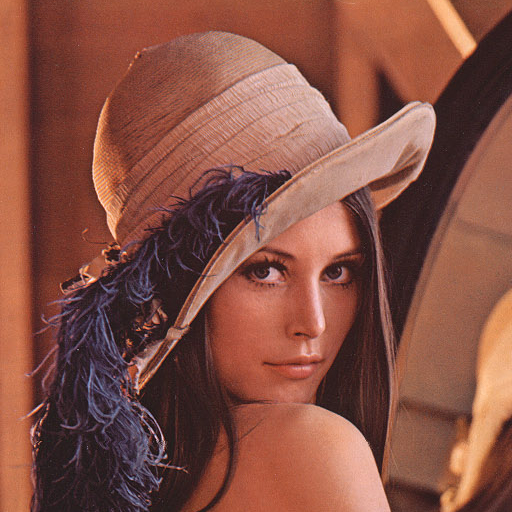
\includegraphics[width=0.4\textwidth]{imagenes/lena32.jpg}\label{fig:f5}}
  \hfill
  \subfloat[LDR]{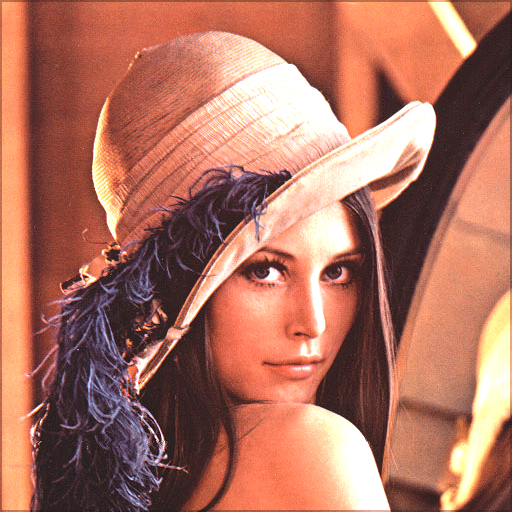
\includegraphics[width=0.4\textwidth]{imagenes/lena32ldr.jpg}\label{fig:f6}}
  \caption{$\alpha$: 255}
\end{figure}


Para reducir errores de redondeo, la division debe será la última operación en realizarse.
El resultado final será saturado de ahi $max$ y $min$ en la primer fórmula.

Además, dado que en los bordes no es posible calcular ldr por la ausencia de vecinos, se devolverá
el valor original. Es decir:

\begin{center}
$O_{i,j}^{K} = I_{i,j}^{K}$ si $i<2 \vee j<2 \vee i+2 \leq tamy \vee j +2 \leq tmax$
\end{center}

(con i indexado a partir de 0)

\subsubsection{Assembler SIMD}

En la implementación de $ldr$ tenemos varios inconvenientes a solventar, pero el principal es el cálculo de la suma. Para lograr aprovechar el paralelismo que ofrece SIMD se realizan varias operaciones.
Para cada fila del cuadrado que supone la sumatoria, se obtienen 4 pixeles en un registro $xmm$ y luego se separan en dos registros diferentes, de manera tal que tengamos el los pixeles $p0$ y $p1$ en uno y $p2$ y $p3$ en otro con cada canal transformado a 16 bits. Para realizarlo se realiza un shuffle para cada caso.\\

Una vez obtenidos los dos registros anteriores, se suman horizontalmente los registros respectivos una vez y se transforma el resultado a 32 bits. Luego se aplican sumas verticales valiendose de un registro de respaldo y varios shifts para eliminar las sumas que no signifiquen en la fórmula.\\

Debido a que la suma que buscamos es de cinco pixeles, se obtiene el 5to pixel en otro registro y se lo opera de manera similar a los anteriores para luego sumarlo a los mismos acumulando la suma de cada fila en el registro particular $xmm0$

\begin{codesnippet}
\begin{verbatim}
.cincoHorizontal:

	; 16  12   8   4   0
	; Li4|Li3|Li2|Li1|Li0
    ;VERSION STANDARD: Con 2 accesos - acceso extra paa el pixel 5
    movdqu xmm13, [rdi + r12*pixelSize] ; Li3|Li2|Li1|Li0

	movdqu xmm9, xmm13
	pshufb xmm9, xmm6 ; 0|0|0|r1|0|g1|0|b1|0|0|0|r0|0|g0|0|b0
	phaddw xmm9, xmm11 ; 0|0|0|0|0+r1|g1+b1|0+r0|g0+b0 -- maximo por w = 510 in []
	pshufb xmm13, xmm7 ; 0|0|0|r3|0|g3|0|b3|0|0|0|r2|0|g2|0|b2
    phaddw xmm13, xmm11 ; 0|0|0|0|r3|g3+b3|r2|g2+b2 -- maximo por w = 510 in []
    punpcklwd xmm9, xmm11 ; r1|g1+b1|r0|g0+b0
    punpcklwd xmm13, xmm11 ; r3|g3+b3|r2|g2+b2
    paddd xmm13, xmm9 ; r3+r1|g3+b3+g1+b1|r2+r0|g2+b2+g0+b0 -- maximo por dw = 1020 in []
    movdqu xmm9, xmm13
    psrldq xmm9, 8 ; 0|0|r3+r1|g3+b3+g1+b1
    paddd xmm13, xmm9 ; r3+r1|g3+b3+g1+b1|r2+r0+r3+r1|g2+b2+g0+b0+g3+b3+g1+b1  -- maximo por dw = 2040 in []
    pslldq xmm13, 8 ; r2+r0+r3+r1|g2+b2+g0+b0+g3+b3+g1+b1|0|0
    psrldq xmm13, 8 ; 0|0|r2+r0+r3+r1|g2+b2+g0+b0+g3+b3+g1+b1
	movd xmm9, [rdi + r12*pixelSize + 16] ; 0|0|0|0|0|0|0|0|0|0|0|0|a4|r4|g4|b4

	pslldq xmm9, 12 ; a4|r4|g4|b4|0|0|0|0|0|0|0|0|0|0|0|0
	pand xmm9, xmm8 ; 0|r4|g4|b4|0|0|0|0|0|0|0|0|0|0|0|0
	pshufb xmm9, xmm7 ; 0|0|0|r4|0|g4|0|b4|0|0|0|0|0|0|0|0
	phaddw xmm9, xmm11 ; 0|0|0|0|r4|g4+b4|0|0 -- maximo por w = 510 in []
	punpcklwd xmm9, xmm11 ; 0|r4|0|g4+b4|0|0|0|0
	psrldq xmm9, 8 ; 0|0|r4|g4+b4
	paddd xmm13, xmm9 ; 0|0|r2+r0+r3+r1+r4|g2+b2+g0+b0+g3+b3+g1+b1+g4+b4 -- maximo por dw = 2550 in []
	movdqu xmm9, xmm13
	psrldq xmm9, 4 ; 0|0|0|r2+r0+r3+r1+r4
	paddd xmm13, xmm9 ; 0|0|r2+r0+r3+r1+r4|g2+b2+g0+b0+g3+b3+g1+b1+g4+b4+r2+r0+r3+r1+r4 -- maximo por dw = 3825 in []
	pslldq xmm13, 12 ; g2+b2+g0+b0+g3+b3+g1+b1+g4+b4+r2+r0+r3+r1+r4|0|0|0
	psrldq xmm13, 12 ; 0|0|0|g2+b2+g0+b0+g3+b3+g1+b1+g4+b4+r2+r0+r3+r1+r4
	paddd xmm0, xmm13 ; suma de la i fila para el pixel ij.

	add r12, r15
	inc r10
	cmp r10, 5
	jl .cincoHorizontal
\end{verbatim}
\end{codesnippet}

Una vez obtenida la suma, que al final tendrá un tamaño de 32 bits, se procede a realizar la fórmula de ldr. 
El primer paso es armar la un registro con el valor de $alfa$ en sus primeras tres posiciones menos significativas que es donde se encontraran los valores de los canales. Asi mismo, se crea un registro con el divisor $max$ en las cuatro posiciones debido a que con el realizaremos la division.\\

Se crea un registro con la suma replicada en las tres posiciones menos significativas y se procede a calcular la fórmula, para lo cual tenemos la siguiente consideración:\\
 
Debido a que, $canal x sumargb x alfa$ cabe perfectamente dentro de un entero de 32 bits (el máximo es $75x255x255x255$ o $75x255x255x-255 = +-1,243,603,125$ $\in$ $[-2,147,483,648$ a $2,147,483,647]$, no se convierte a punto flotante si no hasta la division, por lo tanto será la única operacion de punto flotante del algoritmo, aunque vale mencionar que si por cada pixel, exceptuando las primeras y últimas dos filas y columnas se aplica esta fórmula en total habrá 3$x$(filas-2)$x$(columnas-2) operaciones de punto flotante. Para una imágen de 512$x$512 supone 780300 divisiones de punto flotante, que se asemeja bastante a la cantidad de operaciones de punto flotante de $sepia$.


\begin{codesnippet}
\begin{verbatim}

	pxor xmm13, xmm13
	movd xmm13, ebx
	movdqu xmm12, xmm13 ; 0|0|0|alpha
	pslldq xmm12, 4 ; 0|0|alpha|0
	por xmm12, xmm13 ; 0|0|alpha|alpha
	pslldq xmm12, 4 ; 0|alpha|alpha|0
	por xmm12, xmm13 ; 0|alpha|alpha|alpha

	pxor xmm14, xmm14
	movd xmm14, r13d
	movdqu xmm13, xmm14 ; 0|0|0|max
	pslldq xmm13, 4 ; 0|0|max|0
	por xmm13, xmm14 ; 0|0|max|max
	pslldq xmm13, 4 ; 0|max|max|0
	por xmm13, xmm14 ; 0|max|max|max
	pslldq xmm13, 4 ; max|max|max|0
	por xmm13, xmm14 ; max|max|max|max

	movdqu xmm5, xmm0 0|0|0|0
	pslldq xmm5, 4 0|0|sumargb|0
	por xmm5, xmm0 0|0|sumargb|sumargb
	pslldq xmm5, 4 0|sumargb|sumargb|0
	por xmm5, xmm0 0|sumargb|sumargb|sumargb
	pxor xmm14, xmm14
	movd xmm14, [rdi + r8*pixelSize] ; 0|0|0|0|0|0|0|0|0|0|0|0|a|r|g|b <- get pixel ij
	movdqu xmm0, xmm14 ; 0|0|0|0|0|0|0|0|0|0|0|0|a|r|g|b
	pand xmm0, xmm15 ; 0|0|0|0|0|0|0|0|0|0|0|0|0|r|g|b
	punpcklbw xmm0, xmm11 ; 0|0|0|0|0|r|g|b
	punpcklwd xmm0, xmm11 ; 0|r|g|b
	pmulld xmm5, xmm0 ; 0|sumargb*r|sumargb*g|sumargb*b == 0|sumargb*r|sumargb*g|sumargb*b -- maximo posible por dword 75*255*255 = 4876875 in  [-2,147,483,648 to 2,147,483,647]
	pmulld xmm5, xmm12 ; 0|alpha*sumargb*r|alpha*sumargb*g|alpha*sumargb*b <- puede cambiar el signo segun alpha. -- maximo posible por dword 75*255*255*255 or 75*255*255*-255 = +-1,243,603,125 in  [-2,147,483,648 to 2,147,483,647]
    cvtdq2ps xmm5, xmm5 ; 0|fp(alpha*sumargb*r)|fp(alpha*sumargb*g)|fp(alpha*sumargb*b)
	cvtdq2ps xmm13, xmm13 ; fp(max)|fp(max)|fp(max)|fp(max)
	divps xmm5, xmm13 ; 0|(alpha*sumargb*r)/max|(alpha*sumargb*g)/max|(alpha*sumargb*b)/max
	cvtdq2ps xmm0, xmm0 ; 0|fp(r)|fp(g)|fp(b)
	addps xmm5, xmm0 ; 0|r+(alpha*sumargb*r)/max|g+(alpha*sumargb*g)/max|b+(alpha*sumargb*b)/max
	cvttps2dq xmm5, xmm5 ; cast to dw signed 
	packusdw xmm5, xmm11 ; 0|0|0|0|0|r+(alpha*sumargb*r)/g+max|(alpha*sumargb*g)/b+max|(alpha*sumargb*b)/max
	packuswb xmm5, xmm11 ; 0|0|0|0|0|0|0|0|0|0|0|0|0|r+(alpha*sumargb*r)/g+max|(alpha*sumargb*g)/b+max|(alpha*sumargb*b)/max <- tengo los canales calculados saturados a byte.
	pand xmm14, xmm4 ; 0|0|0|0|0|0|0|0|0|0|0|0|a|0|0|0
	por xmm14, xmm5 ; 0|0|0|0|0|0|0|0|0|0|0|0|a|r+(alpha*sumargb*r)/max|g+(alpha*sumargb*g)/max|b+(alpha*sumargb*b)/max
	
\end{verbatim}
\end{codesnippet}

\subsubsection{C}

Como ya hemos explicado, C carece de paralelismo en las operaciones, por lo tanto tendremos que lidiar de la manera tradicional, obteniendo cada pixel y operando unitariamente. Al final el agoritmo es similar pero con más accesos a memoria para lectura y escritura.

\begin{codesnippet}
\begin{verbatim}

                int i = 0;
                int indexSquare = c - ((cols*2)+2);
                int sumargb = 0;
                
                while (i < 5) {
                    sumargb += src[indexSquare*4];
                    sumargb += src[indexSquare*4+1];
                    sumargb += src[indexSquare*4+2];
                    sumargb += src[indexSquare*4+4];
                    sumargb += src[indexSquare*4+5];
                    sumargb += src[indexSquare*4+6];
                    sumargb += src[indexSquare*4+8];
                    sumargb += src[indexSquare*4+9];
                    sumargb += src[indexSquare*4+10];
                    sumargb += src[indexSquare*4+12];
                    sumargb += src[indexSquare*4+13];
                    sumargb += src[indexSquare*4+14];
                    sumargb += src[indexSquare*4+16];
                    sumargb += src[indexSquare*4+17];
                    sumargb += src[indexSquare*4+18];
                    indexSquare += cols; //siguiente fila.
                    i++;
                }

                float sumargbf = sumargb;
                float alphaf = alpha;
                float maxf = 4876875;
                float b = (float)src[c*4];
                float g = (float)src[c*4+1];
                float r = (float)src[c*4+2];
                unsigned char a = src[c*4+3];

                b = b + (alphaf*sumargbf*b)/maxf;

                b = MIN(MAX(b,0), 255);

                g = g + (alphaf*sumargbf*g)/maxf;

                g = MIN(MAX(g,0), 255);

                r = r + (alphaf*sumargbf*r)/maxf;

                r = MIN(MAX(r,0), 255);

                dst[c*4] = (unsigned char)b;
                dst[c*4+1] = (unsigned char)g;
                dst[c*4+2] = (unsigned char)r;
                dst[c*4+3] = a;
                
\end{verbatim}
\end{codesnippet}

\subsection{Análisis experimental}

En general, al aplicar filtros sobre imagenes, la performance puede verse afectada por varios motivos, como por ejemplo el scheduler del sistema, que puede generar caidas en el tiempo debido a que debe realizar operaciones de mayor prioridad antes de poder retornar al algoritmo. Otras cuestiones pueden estar relacionadas con el acceso a memoria.\\

Como bien se sabe, la mayoria de los procesadores poseen una memoria integrada que es la más rápida luego de los registros, conocida como memoria cache, y que se subdivide en dos niveles: L1 (a su vez subdividida en datos e instrucciones) y L2 para datos. 
La idea de la misma es tener $"$a mano$"$ datos que sean pedidos al sistema, trayendo consigo además los contiguos en un bloque (Nico, revisá si no es mucho humo) de memoria (principio de vecinidad espacial), de manera tal que al consultar por el mismo nuevamente o algún contiguo, se obtenga mucho más rápido desde esta memoria. Pero cuando los mismos no se encuentran, el procesador tiene que buscarlos en la memoria ram, siendo este proceso la causa en la caida de performance que más suele afectar a los algoritmos.\\ 

Este y algunos motivos más serán de estudio en este informe. Para ello introduciremos cada una de las hipótesis que se plantearán en base a lo que cada implementación en particular genere y propondremos un test a realizar, explicando la metodologia para llevarlo a cabo y los resultados obtenidos con las conclusiones que correspondan.\\
 
Además, escogeremos una implementación en particular para llevar a cabo algunos tests especiales que surjan en base a resultados más o menos generales para tener una vision extra de lo que sucede en esos casos.\\

\subsubsection{Metodologias}

Evaluaremos con los distintos tests el rendimiento de cada implementación. El mejor o peor rendimiento de las implementaciones se basa en la toma de tiempos de ejecución. Como los tiempos de ejecución son relativamente pequeños, en general, se utilizará uno de los contadores de performance que posee el procesador. \\

La imágen elegida para los tests será la siguiente: se sube!!.

\begin{figure}
  \begin{center}
	
\includegraphics[scale=0.10]{imagenes/starWars.jpg}
	\caption{La última de Star Wars}
	\label{starwars}
  \end{center}
\end{figure}


INSERTE DATOS DEL PROCESADOR CON COMENTARIO AQUI $\rightarrow$

Para que la cache no influya en cada corrida se implementó un algoritmo sencillo que lo que hará es ocupar la cache L2 antes de cada corrida. Sabiendo que la cache es de 2MB el algoritmo siguiente debería garantizar que la cache se ocupará con información que no altere los resultados de los tests. \\

\begin{codesnippet}
\begin{verbatim}

                char *basura = (char*)malloc(sizeof(char)*2048);
                srand(5);
                int i = 0;
                while (i < 2048) {
                    basura[i] = rand() % 27;            
                    i++;                
                }
                long int suma = 0;
                i = 0;                
                while (i < 2048) {
                    suma += basura[i];   
                    i++;         
                }
                free(basura);

\end{verbatim}
\end{codesnippet}

\pagebreak

\subsection{Hipótesis}


\subsubsection{Aumentando resoluciones}

Nos interesa saber como varia el rendimiento de los algoritmos para cada filtro en sus dos variantes ($asm$, $C$) cuando se varia el tamaño de ~\ref{starwars}.\\

El resultado esperado es que para todos los filtros en ambas versiones el tiempo sea creciente a medida que el tamaño crece. Además, que la version en $asm$ se mantenga por encima de $C$ siempre. \\ 


ESTO VA LUEGO DE REALIZADO EL TEST:

Parámetros del test: 
Cantidad de iteraciones por filtro 10. Aumentos 100x100.
ALFA 100, CORTE: 140 60 0 0

Según nuestra hipótesis, con un aumento de forma cuadratica en el tamaño de las imágenes se obtiene una curva casi cuadratica, pero dado q las imagenes utilizadas poseen más altura que ancho, la curva resultante es más amplia. \\

Luego, en base a esto, planteamos (para el filtro de LDR), que con un aumento solo en el ancho de la imágen, la curva resultante deberia ser una recta. \\

Tambien planteamos que si invertimos el tamaño, haciendo que sea 2160x3840 y generamos los aumentos, el test deberia dar mas cuadratico. \\

Esto se podria expresar matematicamente diciendo que $curva =a*x^2$ con $a>1$ cuando es mas ancha que alta y $a<1$ cuando es mas alta que ancha. \\

Por último observar que en cache se mantiene constante. \\

\subsubsection{Performance: implementaciones y filtros}

La meta principal del informe es comprobar que $asm$ es mejor que la implementación de $C$
Para esto correremos todos los filtros comparando sus versiones de $assembler$, $C$ y además incluiremos $C$ con flags de optimización, en particular $O3$ para ver que tan bien puede optimizar el compilador. \\

El resultado esperado es que $assembler$ debería ser superior, es decir insumir una menor cantidad de ciclos que las otras dos versiones. Aunque no esperariamos un mal rendimiento de $C$ con optimización. \\

ESTO VA LUEGO DE REALIZADO EL TEST:

Parámetros del test: 
Cantidad de iteraciones por filtro-version 20.

Concluimos que assembler es mejor pero que O3 le pega en el palo. \\

\subsubsection{Performance: cropflip vs. cache}

El filtro cropflip parece poseer una particularidad. Utiliza accesos a memoria aleatorios que en principio deberian afectar el rendimiento en cuanto a si los datos pedidos estan cacheados o no. 
Si el corte realizado es muy ancho que alto, por principio de vecinidad espacial, el algoritmo debería tener un buen rendimiento, no así, cuando el corte es mas alto que ancho. \\

Llevaremos a cabo entonces, un test para comprobar si este hecho tiene relevancia, esperando que, verdaderamente sea un factor influyente.
Lo que haremos, como se comentó anteriormente, será limpiar la cache en cada corrida, para que así cada test no se vea afectado por el anterior. Luego esperariamos ver que cuanto más alto que ancho sea el corte peor rendimiento tendrá el algoritmo debido a que como los datos no se encuentran cacheados, tendrá más accesos a memoria ram. \\

ESTO VA LUEGO DE REALIZADO EL TEST:

Parámetros del test: 
Cantidad de iteraciones por filtro-version 20.

Concluimos que salvo por las imagenes mas chicas que no se que goma pasa ahi, el test es constante. Por lo cual la cache no parece ser un factor relevamente en este caso como suponiamos. (HABRIA QUE CORRER ESTE TEST UNA VEZ MAS. AUNQUE YO YA PROBE INCLUSO CON DOS VARIACIONES DEL FLUSHEADOR Y DIO IGUAL)


\subsubsection{Performance: versiones de ldr}

Elegimos el filtro $LDR$ para analizar dos teorias relacionadas a SIMD. 

$a)$ Si igualamos la cantidad de accesos de la version de $assembler$ a la de $C$ aún asi la version de $assembler$ será más óptima.

$b)$ Si en vez de dividir en punto flotante se reemplaza esa seccion de codigo por operaciones con enteros: que version tiene mejor rendimiento? $assembler$ con ops de punto flotante o $assembler$ con ops en enteros?


\begin{codesnippet}
\begin{verbatim}

	;TEST 2: OPERACIONES CON ENTEROS
	pmulld xmm5, xmm0 ; 0|sumargb*r|sumargb*g|sumargb*b == 0|sumargb*r|sumargb*g|sumargb*b -- maximo posible por dword 75*255*255 = 4876875 in  [-2,147,483,648 to 2,147,483,647]
	pmulld xmm5, xmm12 ; 0|alpha*sumargb*r|alpha*sumargb*g|alpha*sumargb*b <- puede cambiar el signo segun alpha. -- maximo posible por dword 75*255*255*255 or 75*255*255*-255 = +-1,243,603,125 in  [-2,147,483,648 to 2,147,483,647]
	; PROBLEM HERE -->;divps xmm5, xmm13 ; 0|(alpha*sumargb*r)/max|(alpha*sumargb*g)/max|(alpha*sumargb*b)/max
    mov r10, rdx ; salvo resto
    xor rdx, rdx
    xor rax, rax
    movd eax, xmm5 ; alpha*sumargb*b
    div r13d ; alpha*sumargb*b/max
    pxor xmm10, xmm10
    movd xmm10, eax ; 0|0|0|alpha*sumargb*b
    pslldq xmm10, 4 ; 0|0|alpha*sumargb*b|0
    xor rdx, rdx
    xor rax, rax
    psrldq xmm5, 4
    movd eax, xmm5 ; alpha*sumargb*g
    div r13d ; alpha*sumargb*g/max
    movd xmm10, eax ; 0|0|alpha*sumargb*b/max|alpha*sumargb*g/max
    pslldq xmm10, 4 ; 0|alpha*sumargb*b/max|alpha*sumargb*g/max|0
    xor rdx, rdx
    xor rax, rax
    psrldq xmm5, 4
    movd eax, xmm5 ; alpha*sumargb*r
    div r13d ; alpha*sumargb*r/max
    movd xmm10, eax ; 0|0|alpha*sumargb*b/max|alpha*sumargb*g/max|alpha*sumargb*r/max
    mov rdx, r10 ; recupero resto
    
\end{verbatim}
\end{codesnippet}

ESTO VA LUEGO DE REALIZADO EL TEST:

Parámetros del test: 
Cantidad de iteraciones por filtro-version 20.
ALFA 100

$a)$ Gana $assembler$. Claramente los accesos no suponen un problema. La diferencia esta en el procesamiento paralelo.

$b)$ Gana con ops en punto flotante: Para este caso particular, al menos, el hecho de tener que dividir cada escalar por separado no supone una ventaja, todo lo contrario. Y al final es mas conveniente operar en punto flotante, dado que ya veniamos procesando en paralelo.
